\chapter{Background}

Before designing the infrastructure, I provide more information to help understand my problem domain. I present information on different topics. First, I talk about Project EPIC and its work on crisis informatics. After that, I present on how REST APIs work and how container orchestration technologis are valuable. Then, I dig deeper into cloud infrastructures, big data storage systems, cloud object storage, and cloud document analysis tools. After that, I talk about microservice frameworks and the differences between monolithic and microservice-based infrastructures. I also explain why I chose microservices for the design of my software infrastructure. 

\section{Project EPIC}

\begin{figure}[htbp]
	\caption{\label{fig:oldepicinfra}
	Project EPIC old software infrastructure diagram .
	}
    \begin{center}
	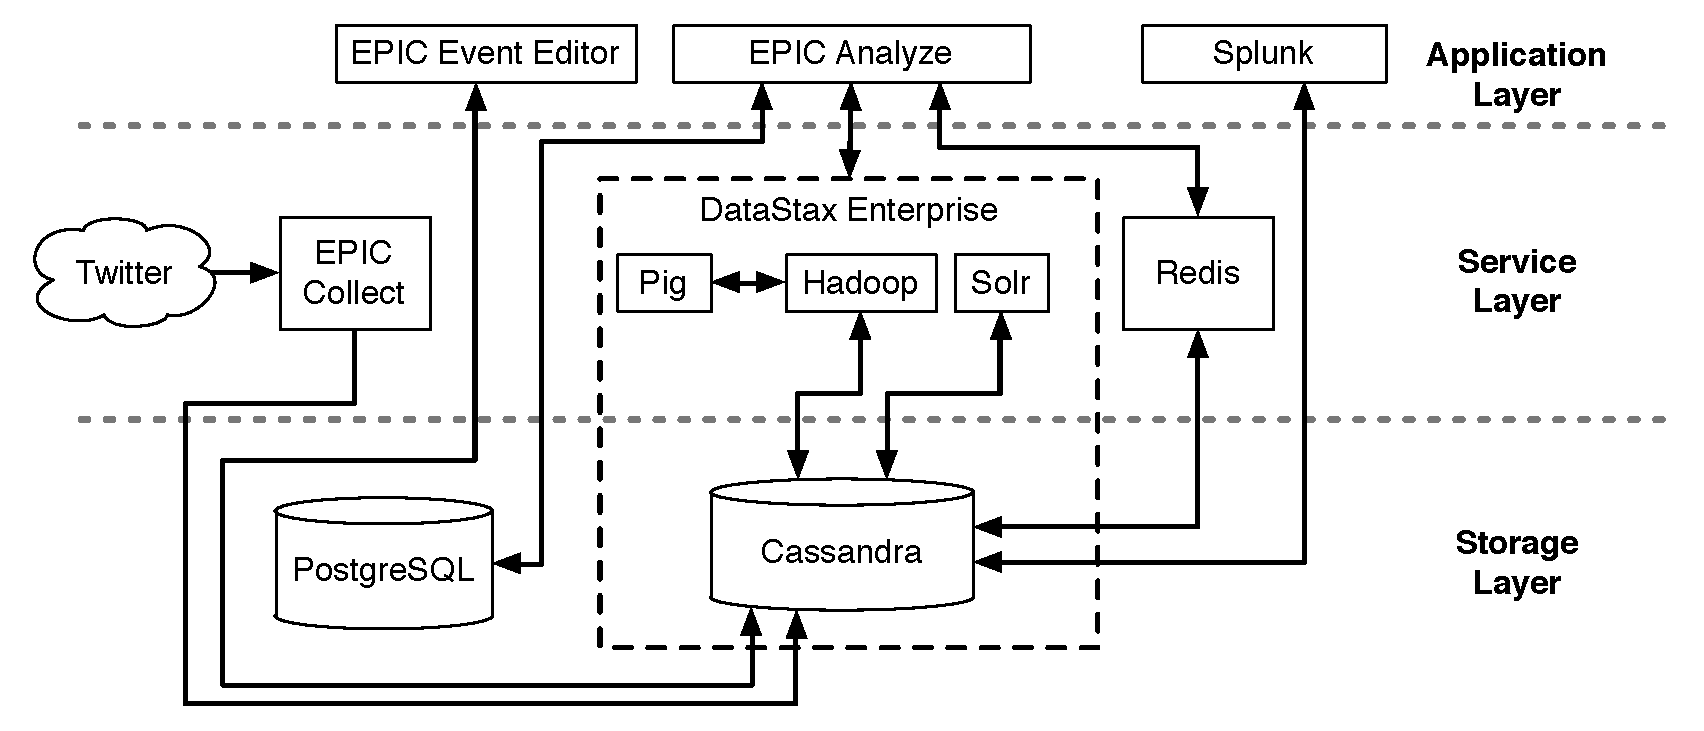
\includegraphics[width=100mm]{figs/old-arch.pdf}
    \end{center}
\label{xfigDiagram}
\end{figure}

Project EPIC (Empowering the Public with Information in Crisis) is a project at the University of Colorado Boulder. It conducts research on crisis informatics, an area of study that examines how members of the public make use of social media during times of mass emergency to make sense of a crisis event and to coordinate/collaborate around an event. Project EPIC has a long history of performing software engineering research. Since 2009, Project EPIC has been investigating the software architectures, tools, and techniques needed to produce reliable and scalable data-intensive software systems, aka big data software engineering\cite{Anderson:2015b}.

When large amounts of data are being collected, software engineers need to focus on structuring it so it is easy to perform analysis. They must work to ensure that the data is easily accessible to analysts. Project EPIC's big data software engineering research has explored these issues in depth during the creation of the previous Project EPIC software infrastructure that consisted of two major components: EPIC Collect and EPIC Analyze. EPIC Collect\cite{anderson2011design,schram2012mysql} is a 24/7 data collection system that connects to the Twitter Streaming API to collect tweets from various crisis events that need to be monitored in real time. Since 2012 to 2018, this software collected tweets with an uptime of 99\% and collected over two billion tweets across hundreds of crisis events. EPIC Collect used Cassandra as its storage layer. This NoSQL database is focused on writes and provided high throughput to handle all incoming tweets. EPIC Analyze\cite{anderson2015design,barrenechea2015getting} is a web-based system that makes use of a variety of software frameworks (e.g., Hadoop, Solr, and Redis) to provide various analysis and annotation services for analysts on the large data sets collected by EPIC Collect. In addition, Project EPIC maintained one machine---known as EPIC Analytics---with a large amount of physical memory to allow analysts to run memory-intensive processes over the collected data. 

The software architecture of EPIC Collect and EPIC Analyze is shown in Figure \ref{fig:oldepicinfra}. Note, this is a logical architecture that does not show how these systems are deployed. For instance, Cassandra was deployed on four machines that run separately from the machines that host the EPIC Collect software, Postgres, Redis, and the Ruby-on-Rails code that makes up EPIC Analyze. In all, the existing Project EPIC infrastructure was distributed across seven machines in a single data center maintained at the University of Colorado Boulder.

\section{REST API}

REST (Representational State Transfer) \cite{fielding2000architectural} is a well known architectural style that defines a set of constraints to be used when designing and implementing a web service. It recommends a pattern for making use of HTTP verbs on URLs that follow certain conventions for designing a natural way to design web services that then provide many of the same benefits provided by the Web itself. REST APIs provide an abstraction to a set of resources that shield the client from the internal representations of the data. Interaction is done through a HTTP request, making it easy to implement web applications thanks to its adoption across the internet. Designed as stateless operations, REST services help separate the user interfaces of clients from underlying technologies.

URIs are used to identify resources. That is, URIs make it possible to find an object in the system. Each URI must be unique for a single resource. A good practice is to format each resource URI in an ordered path structure. A lot of times a request to a service for a particular resource will return hyperlinks to other resources allowing a service to be built around a well-known URI and then letting clients discover other resources via service interactions. Each resource accepts a set of operations that derive from the HTTP operations: GET, HEAD, POST, PUT, PATCH, DELETE, CONNECT, OPTIONS. These can be used in pair with other parameters to execute a variety of actions on a resource. 

RESTful services allow for various CRUD (Create, Read, Update and Delete) operations to be performed easily. Here is a list of some CRUD operations mapped to an example REST service:

\begin{itemize}
    \item List all resources available \textit{GET /notes/}: Note the use of a plural with respect to the resource name as there are multiple notes in the folder. Also, use \textit{/} at the end, as it is functioning like a container or folder in a traditional desktop file system.

    \item Get a representation of a specific resource \textit{GET /notes/1}: This URI and HTTP verb will retrieve a unique representation for a single resource. We do not use \textit{/} at the end as we are accessing a specific resource.

    \item Create a new resource \textit{POST /notes/}: This should add a new element to the list of resources available. If no unique ID is provided, a new ID should be assigned by the web service and returned to the client. 

    \item Remove a specific resource \textit{DELETE /notes/1}: This should remove the specified resource from its containing resource. 

    \item Update a specific resource \textit{PATCH /notes/1}: This should replace the existing resource with the new representation that accompanies this request.

\end{itemize}

These operations can be augmented with parameters. We could add a GET parameter to filter down the results returned when we list all available resources. An example would be to list all notes that have not been archived. We could do so via ‘GET /notes/?archive=false’. This helps us cache future responses if the same filter is used again. These parameters are also useful when searching resources or for any other operations that may filter the result returned to the user. For creating and updating elements, we use the body from the request to include a representation of the object we are creating or updating. 

A common bad practice that should be avoided is using URIs for passing arguments. An example of such is adding the search term into the URI like \textit{GET /notes/search/hello}. This should be avoided since this is a parameter for a function, not a static resource to be retrieved or updated. Instead it should use GET parameters like ‘GET /notes/?search=hello’ as described before. 

For this project, I decided to use REST APIs to overlay an abstraction on top of my underlying infrastructure. Each API exposes a set of resources that allows the user to interact with the collection and analysis infrastructure. This abstraction layer allows changing the underlying infrastructure without affecting its clients. Also, thanks to the separation of data storage and user interface, I can change user interfaces individually independent of the underlying data. This separation allows having developers who are more front-end focused working on the user interface without the need to understand how the underlying system works.

\section{Container Orchestration Technologies}

As containerization technologies became more widely adopted---spurred by a recent migration to designing systems via microservices---large companies needed a way to manage their containers in a more friendly way. Interconnecting containers, managing their deployment, and scaling them to meet demand, were all possible, but were difficult to achieve. As a result, container orchestration systems were born.

To manage containers, these systems add an abstraction layer over containerisation technologies, making life cycle tasks related to containers (create container, launch container, pause container, etc.) easier to perform. There are a several container orchestration systems available at the moment. The most popular are Kubernetes and Apache Mesos.

In this project, I will make use of Kubernetes. The main reason for this is that---thanks to the open source community---it is easier to find tutorials and courses for Kubernetes. In addition, there are a lot of big companies backing this project and contributing to it; this activity provides evidence that this project will be supported well into the future. Finally, there is a lot of companies offering managed clusters on Kubernetes, which helps to migrate an infrastructure built on top if it if there was ever a need.

Google Cloud seems like the best fit to host Kubernetes as it has a managed cluster option that makes it straightforward to install and configure. In addition, thanks to Google being part of the maintenance team for Kubernetes, there is great support for Google Cloud services within Kubernetes.

\section{Cloud infrastructures}

Cloud infrastructures appeared in response to the need for big companies to maintain large sets of machines in their data centers for peak usage of their apps. The first company to create a cloud service division---and the one responsible for the popularization of cloud services---is Amazon. Amazon needed large data centers to be able to process the demand of the U.S. ``Black Friday'' holiday. However, during the rest of the year, they realized that their servers were mostly unused. They created the division of Amazon Web Services  to lease the computational power of those idle machines to external users.

Other cloud providers have appeared over the years. Google Cloud, Azure, and DigitalOcean are examples. With time, their offerings have switched from only leasing computational power to more complex tools. Some services offered by all these companies include managed databases, object storage, machine learning services, and more. Price and service availability is usually similar between them. 

With the rise of these services, software engineers have started to switch design practices to incorporate the cloud. Those architectures are designed to leverage cloud services for a more cost-effective system. Instead of using an in-house managed service they rely on cloud managed services for different pieces of their infrastructure. This allows savings on maintenance as the overall structure is simplified.

\section{Big Data Storage Systems}

For my thesis work, I will be collecting data from Twitter via the Streaming API. This API is limited to provide 1\% of the total tweets generated in Twitter every minute. Based on a report from 2013\cite{tweetsRecord}, I know that rate is approximately 5700 tweets per second on average. As a result, I can calculate the total number of tweets per second that I estimate will flow through my collection infrastructure. That is approximately 57 tweets per second on average as a minimum bound. Since that corresponds to 4.9M tweets/day, I need a data storage technology that scales to handle large data sets. 

Previous studies in Project EPIC pointed to the usage of NoSQL database. However, systems like this can become a huge bottleneck for analysis workloads. Collection storage needs to be separated from analysis storage in order to increase reliability and avoid analysis queries causing a computational bottleneck that can affect the overall performance of the collection pipeline. 

In addition, I believe it is important for the future to keep data in the raw format in which it was received. Storing raw data will allow the evaluation of new tools. In addition, storing unstructured data as documents is better than converting the original format into a specific database representation since Twitter can (and does) change its data structures at any time.  

\section{Cloud Object Storage}

Most cloud service providers offer object storage services, also known as blob storage services. These services are documents stores abstracted as file systems. They provide cheap and reliable file storage. In addition, they provide programmatic ways to add files, download, and list them from code. Cost is based on the total storage needed, which avoids having to pay for extra disk space when its not being used. At the same time, it functions as an abstraction on top of specific disk configurations to simplify management.

Thanks to the file system structure, folders can be used to provide fast filtering by key. This provides guidance in how data should be structured. A clear example of a use case would be to store all tweets collected during a day in a single folder. This would allow us to filter tweets by date quickly. Such keys can be used as a hash table index with prefix look ups. 

Each object stored has internal metadata that works as a means of deciding how to store the file internally as well as how it should be accessed externally. Part of the metadata is used to decide where it should be stored. Files that are accessed rarely can be stored in cold storage for a cheap price. Files that need to be downloaded frequently are usually stored in fast SSD disks to reduce latency. Other options include replicated files across regions allowing the ability to serve files from the closest region to a client. 

Given that in disaster analysis we tend to explore tweets for events individually, individual data elements can sit for a long time without being accessed. This characteristic makes this data perfect for cold storage as it allows to keep costs low while making sure we do not lose any of the data. In addition, having an interface to access the data whenever we really need it, makes this option worth it. 

\section{Cloud Document Analysis Tools} 

Due to the rise of unstructured data, there has been a lot of work within the data analysis world to bring SQL queries to large data sets. Various NoSQL technologies brought parts of SQL to life by providing abstractions on top of their own data access systems. The main issue with those systems is that it needed to have two separate machine clusters, one for collection and one for analysis workloads to ensure the two functions do not overlap with each other or compete for resources. In addition, storage can make use of different formats across the two tasks, which makes it difficult to switch data analysis tools on top of an underlying collection without having to migrate the whole data set to a new format. This can be a problem if a product used is discontinued or slowly abandoned over time.

To address that issue, different alternatives have been created. Hive on top of Hadoop was an attempt of bringing SQL to the MapReduce world. A more recent alternative has been Presto, an interactive query system that can operate quickly at petabyte scale. Created inside Facebook, it is similar to Hive while operating primarily in memory. Its main goal is to allow for interactive queries (i.e. fast response times) to be performed on top of unstructured large data sets. 

Given that analysis workloads are sparse, adapting Presto to use server-less architecture on the cloud makes sense as it can help keep costs low. This allows for computing resources to be created when needed to resolve a query and also allows for high parallelism to reduce the time to compute the result of a query. Cloud services similar to Presto include Athena from Amazon Web Services and BigQuery from Google Cloud. They both offer similar products on a pay-per-data-element-analyzed basis and can be pointed to their own object storage services for data access.

Making use of this type of service, I can keep simple structures of files in object storage while allowing for quick yet complex analysis workloads that are run in parallel without having to support a large infrastructure to do so. This solution can bring great value, especially in fields like disaster analysis where data is not being analyzed continuously. 

An example query that I can do in this system would be to get the number of tweets for each user in a data set and order the result. Using Google BigQuery, I can run this query with a simple SQL query on top of a zipped set of JSON files stored in Google Cloud Storage. 

\begin{table}[htb]
    \caption[Table comparing execution times to data set size]{
    Table comparing query execution times for the top 50 most active users in an event with the size of the overall data set.
	}
    \begin{center}
    \begin{tabular}{|r|r|r|} \hline
	 \textbf{Storage (Gb)} & \textbf{Number of tweets} & \textbf{Query Time (seconds)} \\ \hline 
	
0.03 & 5638 & 2.2 \\ \hline
0.472 & 72027 & 4.1 \\ \hline
2.5 & 408422 & 5.3 \\ \hline
23.1 & 3776311 & 25.2 \\ \hline
204.2 & 34356642 & 111 \\ \hline

	\end{tabular}
   
\end{center}
\label{powertable}
\end{table}


\section{Microservice Architecture}

Microservices is an approach to distributed systems that promote the use of small services with specific responsibilities that collaborate between them, rather than making use of big components with a lot of responsibilities that make interactions more difficult. They are thus more cohesive units of software with minimal dependencies between them. A system designed with loosely-coupled, highly-cohesive software components has always been a highly desirable goal in software design, and microservices help to achieve that goal within distributed software systems\cite{gradybook}.

Compared to monoliths---large software projects with a lot of responsibilities---microservices allow for faster iteration cycles and deployment. This is achieved thanks to the code base for each service being separated. Due to that, developers can works on parts of the bigger system while not overlapping with others. This flexibility also reduces overall system complexity \cite{microservices}. Thanks to the popularization of container orchestrated systems, microservice architectures have become easier to manage and deploy. Container orchestrated systems provide an abstraction that matches really well with microservices. 

Another advantage of microservices architecture is that it allows for different frameworks and languages to be composed into a single system architecture. Even though this can be interesting to accommodate developers, it is also acknowledged that having a really diverse code base can make it complex for a developer to jump between parts of the system. For that reason, it is recommended to maintain a single language and framework when it comes to designing a microservice architecture. It is still interesting to have the option to jump to a new language or framework to use custom features only available within them. An example would be having to create a stateless service that handles a large number of messages. It would be interesting to rely on frameworks and languages focused on parallel processing and message passing to improve performance. For the decision of what language should be the main framework for a given microservice-based architecture, developer adoption, reliability, and ease-of-use should be the principal criteria.  

Finally, microservice architectures allow for different components to be updated over time and optimized independently. This can benefit the whole infrastructure by helping mitigate bottlenecks on a system individually. In addition, given that the structure is loosely coupled, it allows for services to switch their internal implementation while keeping the same external functionality. An example would be to change the database used by a specific service. The service could be replaced fully by itself without affecting the rest of the system. This simplifies the contracts between teams of developers and reduces dependencies to the APIs of other microservices. 

Having small microservices do specific tasks makes development cycles faster and more independent. It also makes incremental deployment much easier and less dangerous. Finally, microservices make it easier to scale software systems since one can individually scale parts of the system depending on their usage

Most languages have frameworks that allow for easy REST microservices implementations to be created. Dynamic languages frameworks work great for prototyping and allow for fast development. However, they can become difficult to manage unless you make sure your code base is extensively tested. Any line of code can fail due to dynamic typing at execution time and this is dangerous in the long term. This makes it dangerous for production systems as you lose the advantage of analyzing the code when compiling. On the other hand, statically compiled languages make for a more reliable code base as it checks types at compilation time. This can make the code more stable and help detect errors on the code base earlier in the process. 

An example of a framework for microservices would be Dropwizard. This framework, based on Java, provides a complete reliable backbone for microservice development. It includes several libraries to handle database connections and other service connections. Its design is also simple enough to work with so that the learning curve is low. 


